%\documentclass[11.5pt]{article}
\documentclass[conference]{sig-alternate-05-2015}

%\usepackage[a4paper,bindingoffset=0.2in, left=1in,right=1in,top=1in,bottom=1in,footskip=.25in]{geometry}

\usepackage{ifpdf}
%\ifpdf 
%    \usepackage[pdftex]{graphicx}   % to include graphics
%    \pdfcompresslevel=9 
%    \usepackage[pdftex,     % sets up hyperref to use pdftex driver
%            plainpages=false,   % allows page i and 1 to exist in the same document
%            breaklinks=true,    % link texts can be broken at the end of line
%            colorlinks=true,
%            pdftitle=My Document
%            pdfauthor=Cashing Group
%           ]{hyperref} 
%    \usepackage{thumbpdf}
%\else 
%    \usepackage{graphicx}       % to include graphics
%    \usepackage{hyperref}       % to simplify the use of \href
%\fi 

%\usepackage{minted} 

\usepackage{times}
\usepackage{epsfig}
\usepackage{tabularx}
\usepackage{color}
\usepackage{xcolor}
\usepackage{xspace}
\usepackage{thumbpdf}
\usepackage{listings}
\usepackage{verbatim}
\usepackage{booktabs}
\usepackage{colortbl}
\usepackage{cleveref}
\usepackage{caption}

%\setlength\paperheight {11in}
%\setlength\paperwidth {8.5in}
%\setlength{\textwidth}{6in}
%\setlength{\textheight}{8in}
%\setlength{\oddsidemargin}{.25in}
%\setlength{\evensidemargin}{.25in}
%\setlength{\headsep}{0in}
%\pagenumbering{arabic}

\let\oldenumerate\enumerate
\renewcommand{\enumerate}{
  \oldenumerate
  \setlength{\itemsep}{3pt}
  \setlength{\parskip}{0pt}
  \setlength{\parsep}{10pt}
}

% Copyright
\setcopyright{acmcopyright}
%\setcopyright{acmlicensed}
%\setcopyright{rightsretained}
%\setcopyright{usgov}
%\setcopyright{usgovmixed}
%\setcopyright{cagov}
%\setcopyright{cagovmixed}


% DOI
\doi{10.475/123_4}

% ISBN
% \isbn{123-4567-24-567/08/06}

\title{Caching Opportunities in Spark Frameworks}

\author{Ahmed M. Abdelmoniem and Bairen Yi\\
Department of Computer Science and Engineering\\
The Hong Kong University of Science and Technology\\
Clear Water Bay, Hong Kong\\
\{amas, byi\}@cse.ust.hk
}

\date{}

\lstset{escapeinside={<@}{@>}}



\begin{document}

\maketitle

\begin{abstract}
Spark Framework and its successors have recently demonstrated its position as a new fault-tolerant ecosystem for large-scale batch data analysis. They have shown to be highly scalable, support coarse-grained fault tolerance and provide easy to learn Application Programming Interface (API).  Most applications are built to execute different jobs on these frameworks where they often share similar work (for instance, several jobs may use the same input data and/or produce the same output data which is used by next job). Hence, we can spot many opportunities to optimise the execution plan performances for majority of batch jobs. In this report, we plan to explore possible caching techniques in the literature for multi-job optimisation specifically for the Spark framework.  We plan to go further and propose a simple yet efficient caching techniques and policies. Our contribution in this project would be surveying the current and recent literature and proposals of caching and optimisation algorithms that given an input batch of jobs, produces an optimal plan while identifying caching opportunities. Our other contribution is proposing a straightforward caching algorithm that would improve batch job's performance. If possible, we will report our experimental results on Spark deployment to demonstrate that our technique would improve the average completion time of Spark jobs.
\end{abstract}

\section{Introduction}
Motivated by lack abstractions for leveraging distributed memory and means of storing intermediate results which would benefit majority of batch processing applications, it was found that many of these applications like logistic regression and interactive data mining involve the reuse of similar intermediate results multiple times and performing almost same operations on them. Hence, they proposed storing these as in-memory JAVA objects to provide a resilient distributed dataset for such queries along with lineage feature for fault recovery. To this end, Apache Spark \cite{Zaharia2012} was proposed as a general purpose distributed data processing framework that provides fault tolerance through the concept of Resilient Distributed Dataset (RDD). An RDD is an immutable representation of a dataset that is either reliable by nature, i.e.\ stored in reliable external storage, or could be computed from the reliable datasets. Instead of storing the actual data, an RDD stores only its lineage information, i.e.\ the source of data and all transformations specified to compute the data. If any transformation fails under fault, Spark can recover by recomputing the dataset using its reliable ancestors. They also provided an API programming interface through Scala Language to ease the implementation of various programming models on top of Spark. The results are quite staggering and show impressive improvements over MapReduce in Hadoop framework. To summarise we were able to identify the following strength and weaknesses of Spark Framework.

\subsection{Spark Strengths}
We could identify the following strengths from Spark Framework which motivated our choice of seeking further improvement of its completion times.

\begin{enumerate}
\item It complements and address a missing feature of the modern large dataset mining applications which is storing intermediate results.
\item It provides an easy programming interface for faster adoption by many application developers and data analytics.
\item It allows for efficient while less storage-wise costly alternative for fault recovery through leveraging lineage of job stages.
\item RDDs are read-only meaning they can be written out in the background without any program pauses or read-write locking mechanisms. This is quite a promising feature for making any caching algorithm tractable.
\item Spark was 20X and 40X faster than Hadoop for iterative and a real-world data analytics as well as it can scan 1 TB dataset with 5-7s latency.
\item The framework has been evaluated in research (controlled environment) as well as in a real application deployment by Conviva Inc and Mobile Millennium Project.
\end{enumerate}
	
\section{Methodology}

A typical Spark program will construct the actions in an incremental way. The user will usually construct the first RDD using an external data source, usually from file systems or databases. A new RDD is constructed, either explicitly or implicitly, for each transformation applied to the existing RDDs. The Spark program will usually end with one or more actions that either prints out the results or stores the transformed data to external storage. All the RDDs will form a Directed Acyclic Graph (DAG) and the output vertices given by these actions will invoke the actual computation for all their RDD dependencies.

However, the current implementation of Spark evaluates each action as a single Spark job. For Spark programs that contain multiple jobs, we can reduce the computation and storage overhead if the dependency graphs for different jobs share a common substructure. Intuitively, if an RDD is a dependency for multiple Spark jobs, it will be beneficial to avoid re-computation by caching the computed result after its first evaluation. Conversely, if an RDD is a dependency for only a single Spark job, its results will not be reused and its cache could be eliminated after computation to save the storage space.

The following code snippet shows a possible caching optimisation opportunity in the execution of this job:

%\begin{minipage}[c]{\columnwidth}
\begin{lstlisting}[frame=single, caption=Possible Caching Example, label=code:example, breaklines=true]
val lines = spark.textFile("hdfs://inputData")
val num_error_php = errors.filter(_.contains("php")).count()
val num_error_mysql = errors.filter(_.contains("mysql")).count()
val errors = lines.filter(_.startsWith("ERROR"))
<@\textcolor{red}{errors.cache()}  $\leftarrow$  this is where the caching kicks in@>

<@\textcolor{red}{Cashed version of errors dataset can be used in two different jobs}@>
val num_error_php = errors.filter(_.contains("php")).count()
val num_error_mysql = errors.filter(_.contains("mysql")).count()
\end{lstlisting}
%\end{minipage}

Note that the last two variables specify two independent Spark jobs. The line of code with an arrow here is important because without it, the first two lines of code will evaluate each time for the counting task. However, after the multi-job optimisation, the caching statement should be injected to the user program without manually specifying it as shown in Figure~\ref{fig:example}.

\begin{figure}[htbp]
	\centering
		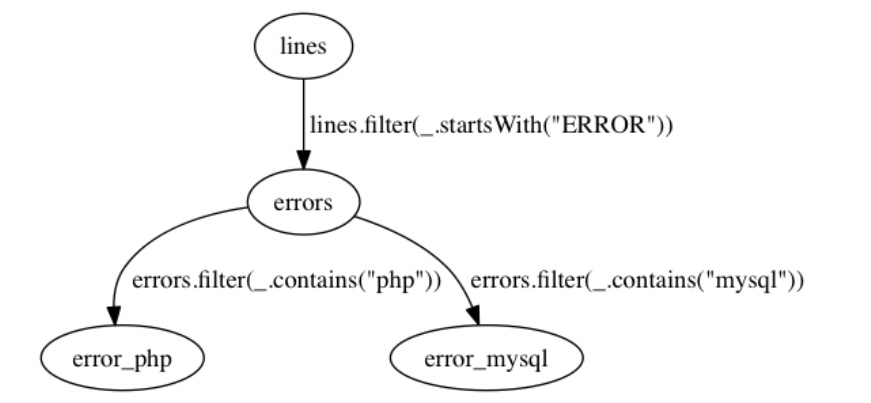
\includegraphics[width=0.95\columnwidth]{images/1.JPEG}
	\caption{Injection of caching mechanism into the jobs execution path of spark}
\label{fig:example}
\end{figure}

\subsection{Data Flow Analysis}

Internally, Spark program instantiates an instance of Java class \texttt{T} that is a subclass of the base class \texttt{org.apache.spark.rdd.RDD} for each transformation. The constructor of the base class consists of two arguments: a sequence of its dependencies \texttt{deps}, and a Spark context singleton. While the latter one is of little interest, the first argument stored in the private field \texttt{dependencies\_} of the base class will be used in runtime to analyze the dependency graph. However, there are two reasons why this information is not useful to our analysis: (1) the subclass could override this behavior by providing an alternative implementation of \texttt{getDependencies()} method, which is a public accessor of \texttt{dependencies\_}; (2) type of field \texttt{dependencies\_} is \texttt{Seq[Dependency[T]]}, an generic container type and its actual content is difficult to be revealed in the compile-time.

Therefore we have to take an alternative approach and analyzing the dependencies by only inspecting the code instead of looking into the content of variable \texttt{deps}. When programming on top of Spark, Spark users usually implicitly construct RDDs by facade methods like \texttt{sc.textFile} or the transformation methods of RDD, instead of manually instantiating RDDs by themselves. The def-use chain of RDD variables in transformation methods reveals data flow dependencies \texttt{dfdeps}, which may not be the same of the accurate dependencies \texttt{deps} that only available at run-time. However, one key observation is that \texttt{deps} is always a subset of \texttt{dfdeps}. In other words, the inference from data-flow dependencies is not sound in the sense that an RDD \texttt{u} in the data-flow dependencies of RDD \texttt{v} does not imply \texttt{u} is an actual DAG dependency of \texttt{v}; but it is complete such that if the value of \texttt{u} does not propagate to instantiation of \texttt{v} in the user program, \texttt{u} is certainly not an actual DAG dependency of \texttt{v}.

In practice, it is difficult to avoid inaccurate possibilities given existence of a variety of control flow constructs, e.g. branching, switching, and loops. Therefore we accept this limitation at a price of static analysis, which does not involve actually running of the program. On the other hand, we will try to quantify the actual precision of the dependency analysis, and compare against the benchmark caching policy, i.e. blindly taking all previous defined RDDs as dependencies without doing data-flow analysis.

Another limitation is from the case where there might be more than one variables in the user program that represent the same RDD in terms of materalization, e.g. reading the same input from disk multiple times, or apply semantically equivalent mapper/aggregation functions more than once to the same dataset, yielding seemingly different results. This limitation is also impossible to avoid in Spark since there is no algorithm that is guaranteed to halt for equivalence relation detection between two arbitrary functions (as permitted in Spark), while it is possible in more restricted form, i.e. SQL, to detect common sub-expression across multiple queries.

The complete design works as follows: each Spark RDD is represented as a immutable variable in the Scala program, either explicitly declared using \texttt{val} keyword or implicitly declared in the return value of chaining method calls. The dependency graph of all RDDs is isomorphic to the data flow graph of RDD variables, which is available at compile-time when constructing the def-use chain for each of the program variable representing an RDD. After merging the dependency graphs of all output into a single monolithic dependency graph, possibly after a pruning to paths that do not lead to an output, the out degrees of the intermediate nodes in the graph will be used to determine whether an alternative caching policy other than the default one could be applied at this point, namely by specifying the priority of caching the intermediate nodes.in descending order.

\section{Related Work}
A number of recent works addressed this shortcoming to improve the execution time and reduce resource usage to be able to pack more jobs within the cluster. \cite{Wang:2013du} proposed two new techniques for multi-job optimization targeting the MapReduce framework. A grouping technique to merge multiple jobs into a single job via sharing both the scan operation of input file and the communication of the common map output. And a materialization technique that share input/ouput through partial materialization of the map output of some jobs. They achieve this by constructing an optimal execution plan by partitioning jobs into groups and assign necessary processing to each group. Figure~\ref{fig:multijob} shows that to achieve map-phase grouping by generating the map output $M_i$ for $J_i$ and at the same time a partial map output $(M_j/M_i^{A_j})$ for $J_j$. In such case, the remaining map output of $J_j$ is not generated as it can be derived from $M_i$ output (i.e.\ , $M_{i,j}$). This technique only  requires two jobs $J_i$ and $J_j$ to satisfy the condition $K_j \in K_i$ (i.e\ , the keys of job j is a subset of identifying keys of job i). On the other hand, materlization works by processing the jobs in a specific sequence such that the map outputs of some of the preceding jobs can be materialized and used by the succeeding jobs in the sequence (\textbf{which is the approach we adopt to achieve benefits of caching}). For Map output materlization during job $J_i$, the map input file F is read to compute both the map output $M_i$ for $J_i$ and $M_j$ for $J_j$. $M_j$ is materialized to the distributed file system (DFS) to be used later for processing $J_j$ which would save time scanning the input file twice. Additionally, reduce sharing is achieved if and only if $K_j \in K_i$ where the map output $M_i^{A_j} \bigcap M_j$ in the reduce phase of $J_i$ is materialized which can be used later by the reduce phase of $J_j$. This approach saves the sorting and communication cost of the map output $M_i^{A_j} \bigcap M_j$ during $J_j$ processing.

\begin{figure}[htbp]
	\centering
		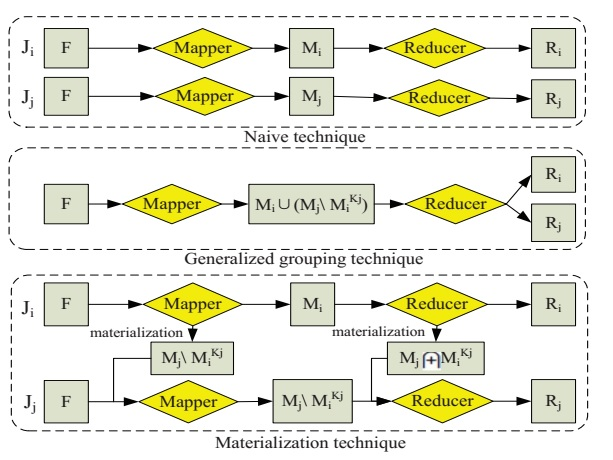
\includegraphics[width=0.95\columnwidth]{images/2.jpeg}
	\caption{The proposed Multi-Job optimization techniques}
\label{fig:multijob}
\end{figure}

\bibliographystyle{abbrv}
\bibliography{../reference}
\end{document}
